\documentclass[11pt,letterpaper]{article}
\usepackage[margin=.65in,headheight=16pt,headsep=14pt,footskip=23pt]{geometry}
\usepackage[T1]{fontenc}
\usepackage{helvet}
\renewcommand{\familydefault}{\sfdefault}
\usepackage{tikz,array,tabularx,fancyhdr,amsmath,amssymb}
\usetikzlibrary{arrows.meta}
\usepackage[hidelinks]{hyperref}
\pagestyle{fancy}\fancyhf{}
\fancyhead[L]{\small Week 56 / Corners of a solid / Adult guide}
\fancyfoot[L]{\scriptsize Bellingham Math Circle / Week 56 / N56-FAC-v1}
\fancyfoot[R]{\scriptsize\thepage}
\renewcommand{\headrulewidth}{.35pt}\renewcommand{\footrulewidth}{.25pt}
\setlength{\parindent}{0pt}\setlength{\parskip}{6pt}
\renewcommand{\arraystretch}{1.22}
\newcolumntype{Y}{>{\raggedright\arraybackslash}X}
\newcommand{\titleline}[1]{\par{\Large\bfseries #1}\par\vspace{4pt}}
\newcommand{\sub}[1]{\par\vspace{3pt}{\bfseries #1}\par}
\newcommand{\hints}[3]{\textbf{Hints, in order.} (1) #1 (2) #2 (3) #3\par}
\newcommand{\degc}{^{\circ}}
\begin{document}
\titleline{The mathematical destination}
\textbf{Euler's formula: $V-E+F=2$. Total angular defect: $720\degc$, or two full turns.} These facts apply to every finite, closed convex solid with plane polygon faces in this packet. $V$, $E$ and $F$ count the assembled surface, including hidden faces. The faces meet along whole edges, each edge belongs to exactly two faces, and the surface has no boundary or holes. Faces are disks; around each vertex the faces form one circular neighborhood.

The counting theorem also holds for a finite cellulation of a sphere with these incidence conditions. For the angle theorem, the cells must be actual planar polygons with consistent corner angles. Such subdivisions can add counted vertices that are not geometric corners of the solid.

\textbf{At a vertex, defect $=360\degc-$ the sum of its plane face-corner angles.} This is the missing angular sector when the corners are laid flat. It is not the angle between two faces, the size of a paper gap in square centimeters, or the turning of an outline. A genuine convex corner has positive defect. A point added inside a face or along an unchanged edge has zero defect: its incident angles still total one full turn.

\textbf{Local fans and whole solids answer different questions.} In Problem 3 the four positive-gap groups can close into pointed corners with no inward dents; the two zero-gap groups close flat. Positive gap is a necessary condition for a genuine convex corner, but an arbitrary collection of such fans need not assemble into a whole closed convex solid. Problem 9 determines counts under its stated whole-solid assumptions; the two particular solids do exist.

\textbf{Limits.} An opened surface has boundary: the opened drawings in Problem 7 have $V-E+F_{\rm bounded}=1$. They are views preserving assembled connections, not cut-apart nets. A sphere's formula cannot simply be used on a box with a missing face, a cylinder band, or a donut. For a closed polygonal manifold surface the angle cancellation gives total signed defect $360\degc(V-E+F)$; a torus has Euler count 0. Its concave corners may have negative defects. No holed model is needed for this visit.

\sub{What children are meant to discover}
Pairing face sides makes one edge; face corners gather in different numbers at vertices. Different solids have the same alternating count and the same total gap. Redrawing a surface changes its inventory without changing these totals. Physical trials are \emph{experiments}; a pattern suggested by them is a \emph{conjecture}; the tree reduction and face-angle argument are \emph{explanations} for all objects in the stated domain.

\begin{tabularx}{\linewidth}{|p{2.15cm}|Y|Y|}\hline
Entry & Prerequisites & A worthwhile result this visit\\\hline
Optional K--1 & Adult reads/records; child aligns dots and sides, handles a fan and chooses comparisons. No degree arithmetic. & Child distinguishes a flat closure from a folded corner and can show the difference.\\\hline
Grades 2--5, pp.1--6 & Count to 24; retain one marked model; short adult-read text. Pp.4--6 add multiples of 60/90, subtraction from 360, and multiplication, with support. & Check several models or fans, notice an incidence rule or a repeated total.\\\hline
Grades 4--5, pp.7--9 & Connected drawings, loops, trees; count differences; polygon angles and multiplication/division. Mathematician available. & Explain one invariant, or solve a reverse inventory. Later visits can complete the proofs.\\\hline
\end{tabularx}

\newpage
\titleline{Preparation for eleven children and three adults}
The group is KK11 / 3333 / 445. Keep the parent at the younger table, the second mathematician at the four third graders, and the organizer at the upper trio. The five working groups are two younger pairs, two middle pairs, and one upper trio. Materials stay at their table; models rotate between its pairs.

\begin{tabularx}{\linewidth}{|p{4.25cm}|Y|}\hline
Print single-sided, US Letter, 100\% & Copies and use\\\hline
\texttt{materials.pdf}, pp.1--2 & 3 copies of each page: one cube, tetrahedron, octahedron and prism per table. 6 cardstock sheets.\\\hline
\texttt{materials.pdf}, pp.3--4 & 6 copies of each page: three complete table sets, two extra fan sets, one spare fan set. 12 cardstock sheets. Assemble only 3 of the 6 pyramid nets; retain the others flat.\\\hline
\texttt{students.pdf}, p.3 & 2 copies for younger pairs, adult read.\\\hline
\texttt{students.pdf}, pp.1--6 & 2 copies per page for middle pairs; give one page at a time.\\\hline
\texttt{students.pdf}, pp.1--9 & 1 shared working copy for upper trio, plus 1 complete spare packet for all tables. Upper pages may stay in reserve.\\\hline
This guide & 3 copies, one per adult.\\\hline
\end{tabularx}
Totals: \textbf{18 cardstock sheets}, \textbf{32 student sheets}, and 3 guides. The active materials are \textbf{15 closed models} (3 of each of five kinds), \textbf{40 triangle pieces, 40 square pieces, 10 circles}. The spare fan set adds 8 triangles, 8 squares and 2 circles. Every working group gets 8 of each polygon and 2 circles. Pairs reuse pieces between trials; they do not need six permanent fans.

\sub{Cut, crease, close, label}
Adults cut and assemble the 15 models before class: 84 polygon faces across them. Nets have \textbf{30 mm face edges}, \textbf{6 mm tabs} with 4 mm tapered ends; circles are \textbf{80 mm across}. Measure the 30 mm bar on material p.1 before cutting. Cut solid outer lines, preserve tabs, crease dashed lines, and put tabs inside. Match both copies of each seam letter and the small blue vertex numbers. Large numbers identify faces. Close bottom faces too. The three five-model sets have 72 tabbed closing seams in total; keep extra tape for reinforcement.

Cut the fan pieces and circles, keeping their marked dots. Use thin removable tape as hinges; join sides without changing polygon shape. Prepare about \textbf{48 short hinge strips}: up to 5 joins for a six-triangle fan and 3 for a four-square fan per set, including the spare set. Final closing seams can use fresh removable strips. Supply \textbf{4 rolls of tape} (one for preparation, one per table), 3 adult scissors, 12 pencils, 3 trays, 3 whiteboards and 3 pens. Put 30 small removable counting marks per table (90 total); count one kind at a time and reuse them. Small marks must not hide the printed corner/seam labels.

For Problem 6, use clear removable tape on the cube as an erasable drawing surface; prepare one pen per table. Reset it completely between the three cases. A drawn line becomes a counted subdivision only for this task. Tabs, tape seams and wrinkles never supply extra faces.

\sub{Physical checks still to perform}
\textbf{Folding, print-scale checks on real paper, tape stiffness, fit, preparation time, handling, staffing and classroom timing have not been rehearsed. All activities are unpiloted.} Before class, assemble one of each model at actual scale; check matching labels, stable closure, readable hidden faces and usable 6 mm tabs. Rehearse making/unfolding six-triangle and four-square fans; verify hinges flex without stretching faces and marks peel cleanly. Square far corners extend slightly beyond an 80 mm circle; the circle measures a turn, not piece containment. Test both younger pairs with one adult reading/recording. Time this preparation; reserve an evening, not the opening minutes of the meeting. Digital dimensions and incidence checks do not prove physical readiness.

\newpage
\titleline{The hour and the shared launch}
\begin{tabularx}{\linewidth}{|p{2.1cm}|Y|}\hline
0--5 minutes & Running around or movement, then settle at the three fixed tables.\\\hline
5--8 & Let every group handle a closed cube and loose face pieces briefly. Gather for the shared action below.\\\hline
8--43 & Work in pairs/trio. Allow substantial time on models or fans; distribute another page only when children want its question.\\\hline
43--53 & Continue the chosen investigation, a readiness-dependent extension, or a fallback below. No requirement to finish pages.\\\hline
53--60 & Each table shows one example. Ask: ``What changed, and what stayed the same?'' Keep the model/drawing with its claim.\\\hline
\end{tabularx}

\sub{Two or three minutes with actual assembled objects}
After handling, hold a closed cube. Say: ``This whole flat patch is one face. These two face sides meet along one edge.'' Trace a real seam once, then touch the corner where its endpoint meets the other faces: ``These face corners meet at one vertex. We count the assembled place once.'' Ask one child to choose another edge and place one removable mark on it. Let the child turn the model to check that the same edge has not been marked twice. Leave inventories to the children.

Next place a loose equilateral triangle's marked dot at the center of an 80 mm circle. A child aligns a second marked dot at the same center, puts a whole side against the first triangle's side, and tapes that join. Say: ``The faces keep their shape. This is an open fan. The part of the turn between the free sides is its gap.'' Trace the missing sector. Do not bend paper faces to force a different angle. The two-triangle example is not one of Problem 3's target groups.

\begin{center}
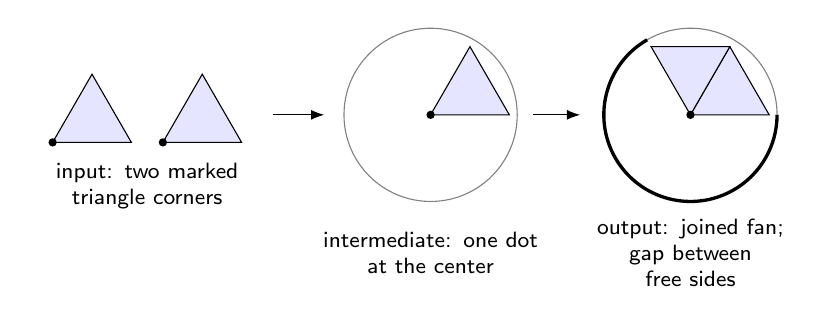
\begin{tikzpicture}[x=1cm,y=1cm,font=\small]
\draw[fill=blue!10] (0,0)--(1,0)--(.5,.866)--cycle;
\draw[fill=blue!10] (1.4,0)--(2.4,0)--(1.9,.866)--cycle;
\fill (0,0) circle (1.5pt);\fill (1.4,0) circle (1.5pt);
\node[align=center,text width=2.8cm,font=\footnotesize] at (1.2,-.55) {input: two marked\\triangle corners};
\draw[-{Latex}] (2.8,.35)--(3.45,.35);
\begin{scope}[shift={(4.8,.35)}]
\draw[gray] (0,0) circle (1.1);
\draw[fill=blue!10] (0,0)--(1,0)--(.5,.866)--cycle;
\fill (0,0) circle (1.5pt);
\node[align=center,text width=2.8cm,font=\footnotesize] at (0,-1.75) {intermediate: one dot\\at the center};
\end{scope}
\draw[-{Latex}] (6.1,.35)--(6.7,.35);
\begin{scope}[shift={(8.1,.35)}]
\draw[gray] (0,0) circle (1.1);
\draw[fill=blue!10] (0,0)--(1,0)--(.5,.866)--cycle;
\draw[fill=blue!10] (0,0)--(.5,.866)--(-.5,.866)--cycle;
\draw[very thick] (120:1.1) arc (120:360:1.1);
\fill (0,0) circle (1.5pt);
\node[align=center,text width=2.8cm,font=\footnotesize] at (0,-1.75) {output: joined fan;\\gap between free sides};
\end{scope}
\end{tikzpicture}
\end{center}

\sub{Who does what}
Younger and middle pairs alternate handler and checker/recorder. At the upper table, rotate builder, checker and recorder among all three children. An adult may read or write a child's report; the child still chooses the next fan/model, makes an attempt, and checks it. If the adult is choosing and performing every comparison, pause that route and return to handling or sorting.

\sub{First routes and fallbacks}
\textbf{Younger:} Problem 3 orally, with three versus six triangles or three versus four squares first; children may then choose other groups. Skip all degree arithmetic. Fallback: one child builds a fan, the partner predicts flat or pointed closure and tests it, then swap. \textbf{Middle:} Problems 1--3 are the core; 4--5 continue the gap discovery if arithmetic is manageable. Fallback: touch a model's vertex and reconstruct its fan. \textbf{Upper:} choose 1--2, 4--6 as concrete preparation; 7, 8 or 9 can each occupy another visit. Fallback: propose a surface redrawing and challenge the partner to account for its count changes.\par
If a child loses the rule, return to one real shared edge or the two-triangle worked visual; do not solve the whole inventory for them.

\newpage
\titleline{Problems 1--2: assembling the inventory}
\sub{Problem 1 / student p.1 / concrete core}
Children turn the four closed models and find vertices, edges and faces. They can divide the models between pairs, then pool checked counts. A drawing's dashed lines are hidden edges, not extra edges. Counting only what a perspective picture shows will miss faces and corners; keep the real models beside the records.

\begin{center}
\begin{tabular}{|l|r|r|r|r|}\hline
Closed model & $V$ & $E$ & $F$ & $V-E+F$\\\hline
Cube & 8 & 12 & 6 & 2\\
Regular tetrahedron & 4 & 6 & 4 & 2\\
Right triangular prism & 6 & 9 & 5 & 2\\
Regular octahedron & 6 & 12 & 8 & 2\\\hline
\end{tabular}
\end{center}
The prism has two triangular ends and three square side faces. The octahedron has four triangular faces above its four-vertex middle ring and four below; the top and bottom are vertices, not faces. Use one list at a time: first mark all faces, remove marks, then edges, then vertices. The printed blue vertex identities provide a check without requiring three simultaneous tallies.

\hints{``Can you turn it over and touch a face we have not marked?''}{Have one child mark a feature while the partner checks whether it is already marked.}{Split the object into a top, bottom and middle ring, or two ends and their joining edges; combine those disjoint parts.}
If counting all four models becomes bookkeeping, keep two contrasting ones (cube and octahedron) and return to the others later. The different inventories will matter in Problem 6; discovering every entry immediately is not compulsory.

\sub{Problem 2 / student p.2 / concrete core}
Children compare separate face sides/corners with assembled edges/vertices and seek a rule. They can put two loose sides against one model edge before doing any multiplication.

\begin{center}
\begin{tabular}{|l|r|r|r|r|}\hline
Faces before assembly & Sides & Edges & Corners & Vertices\\\hline
6 squares: cube & 24 & 12 & 24 & 8\\
4 triangles: tetrahedron & 12 & 6 & 12 & 4\\
2 triangles, 3 squares: prism & 18 & 9 & 18 & 6\\
8 triangles: octahedron & 24 & 12 & 24 & 6\\\hline
\end{tabular}
\end{center}
\textbf{Rule: divide the separate side count by 2.} Every assembled edge has one side from each of exactly two incident faces. A child can explain, ``I counted each edge from both its faces, so each was counted twice.'' This uses closure and the ordinary two-face seam assumption.

\textbf{Separate face corners alone do not determine $V$.} Cube and octahedron both supply 24 face corners. The cube gathers three at each of 8 vertices; the octahedron gathers four at each of 6. Tetrahedron and prism happen to have three face corners at every vertex. Division by 3 works there but is not a general rule. The pyramid later has both three-corner and four-corner vertices.

\hints{``Put two face sides against this one seam. How many sides became one edge?''}{Compare the two rows that both have 24 separate corners.}{Touch an octahedron vertex and gather its four face corners; compare a cube vertex's three.}
For a younger child, the side-pairing action and this counterexample can be spoken and shown. Do not require a completed multiplication table before offering the fans.

\newpage
\titleline{Problems 3--4: local gaps and whole turns}
\sub{Problem 3 / student p.3 / fan core at all tables}
For each printed group, children join marked corners at one point, lay the open fan flat, and draw its missing angular sector. Then they test whether the free sides can meet in a pointed corner with no inward dents, or close flat with no gap. Adjacent face sides meet along their whole length; no stretching, overlap or tearing supplies a legal closure.

\begin{center}
\begin{tabular}{|l|r|r|l|}\hline
Group & Angle used & Gap & Closure without inward dents\\\hline
3 equilateral triangles & $180\degc$ & $180\degc$ & Pointed\\
4 equilateral triangles & $240\degc$ & $120\degc$ & Pointed\\
5 equilateral triangles & $300\degc$ & $60\degc$ & Pointed\\
6 equilateral triangles & $360\degc$ & $0\degc$ & Flat\\
3 squares & $270\degc$ & $90\degc$ & Pointed\\
4 squares & $360\degc$ & $0\degc$ & Flat\\\hline
\end{tabular}
\end{center}
All six groups can lie flat as \emph{open} fans. The distinction is what happens when the free sides \emph{meet}. Positive-gap fans can form convex cones locally; they need not make a complete solid. A six-triangle pleated point can have inward folds, so check the no-dents condition.

\hints{``Can you keep every dot on this one center and make neighboring sides touch?''}{``Lay it flat again. Where is the missing part of the circle?''}{``Bring just the two free sides together. Does it stay flat, lift to a point, or need an inward fold?''}
For K--1, children choose, build/test and point to the gap; the parent records. Start with a clear contrast, then let them choose further groups. A square's far corner beyond the circle is harmless: its angle at the center matters. Stop if recording takes over; save a fan without degree values.

\sub{Problem 4 / student p.4 / arithmetic continuation}
Use the page's two-triangle worked example before subtraction. Children reconstruct a model vertex with loose corners, find its gap, then combine the gaps of all its vertices. Each of these four models has one vertex type.

\begin{center}
\begin{tabular}{|l|r|l|r|r|}\hline
Model & $V$ & Face corners at a vertex & Gap & Total\\\hline
Cube & 8 & 3 squares: $270\degc$ & $90\degc$ & $720\degc$\\
Tetrahedron & 4 & 3 triangles: $180\degc$ & $180\degc$ & $720\degc$\\
Triangular prism & 6 & 1 triangle, 2 squares: $240\degc$ & $120\degc$ & $720\degc$\\
Octahedron & 6 & 4 triangles: $240\degc$ & $120\degc$ & $720\degc$\\\hline
\end{tabular}
\end{center}
All four totals are \textbf{two full turns}. The triangular prism is not a four-triangle vertex even though its gap equals the octahedron's. Children should discover the equality from different local arrangements.

\hints{``Touch one vertex and show its face corners with these loose pieces.''}{``How much of one turn do they use? What remains from 360 degrees?''}{Use the marked vertex count from Problem 1; make one copy of that gap per vertex on spare paper and combine them.}
If degree arithmetic is tiring, the adult can record the calculation after the child chooses the corners and identifies the missing sector. Keep their mathematical choice intact. The repeated total is evidence for a conjecture; it is not yet a proof for all solids.

\newpage
\titleline{Problems 5--6: unequal corners and redrawings}
\sub{Problem 5 / student p.5 / further concrete work}
Children use the square pyramid to find a total when the vertices are not all alike. Its four side faces are equilateral triangles; do not substitute an arbitrary taller pyramid whose triangles have different angles.

\begin{center}
\begin{tabular}{|l|r|l|r|r|}\hline
Vertex type & Number & Corners meeting there & Gap each & Subtotal\\\hline
Top & 1 & 4 triangles: $240\degc$ & $120\degc$ & $120\degc$\\
Base corner & 4 & 1 square, 2 triangles: $210\degc$ & $150\degc$ & $600\degc$\\\hline
\end{tabular}
\end{center}
Total $=120\degc+4(150\degc)=720\degc$. Inventory $(V,E,F)=(5,8,5)$. A unit square base and apex above its center at height $1/\sqrt2$ realize these equilateral side faces, so the model specification is consistent.

\hints{``Touch the top, then a base corner. Do the same faces meet there?''}{Build one fan for each of the two types, including the bottom square at a base corner.}{Count how many of each type occur before combining their gaps.}
If children multiply one gap by five, let them compare their chosen fan with the other vertex type. Do not replace the unequal case with another equal-vertex model: it supplies the reason for the general angle accounting later.

\sub{Problem 6 / student p.6 / upper concrete core or return visit}
First compare the Problem 1 inventories: all four give $V-E+F=2$. Then children draw each of the three printed changes on an otherwise original cube. \textbf{Erase the previous change before beginning another.} The following rows are independent, not cumulative.

\begin{center}
\begin{tabular}{|l|r|r|r|r|r|}\hline
Closed cube surface & $V$ & $E$ & $F$ & $V-E+F$ & Total gap\\\hline
Original & 8 & 12 & 6 & 2 & $720\degc$\\
One face diagonal & 8 & 13 & 7 & 2 & $720\degc$\\
Face center and 4 lines & 9 & 16 & 9 & 2 & $720\degc$\\
One point along an edge & 9 & 13 & 6 & 2 & $720\degc$\\\hline
\end{tabular}
\end{center}
The diagonal adds one edge and one face. The center adds one vertex, four edges and three faces (four triangular pieces replace one square). The edge point adds one vertex and one edge because one old edge becomes two; it appears in both incident face boundaries. The faces themselves are not split.

\textbf{No new vertex can acquire nonzero gap while this cube's shape stays fixed.} At the face center, four right angles total $360\degc$. At an inserted edge point, each adjacent face supplies a straight $180\degc$ angle, again totaling $360\degc$. Old cube vertices retain $90\degc$ defect: drawing lines merely divides their existing plane angles. The total is unchanged.

\hints{``Keep the model unchanged. Which old pieces did your new line actually split?''}{Count the before/after changes rather than recounting the whole cube; trace both faces at the inserted edge point.}{Lay its incident corners flat: does a new point inside a face or along an edge leave a missing sector?}
If children are struggling, keep the diagonal case and its cancellation, then return to center/edge points later. If they want more, let them invent a redrawing and predict the changes before marking it; intersections count as vertices only when the surface is consistently subdivided there. Do not silently combine crossings with unsplit edge segments.

\newpage
\titleline{Problem 7: reduce an opened drawing to a tree}
\sub{Student p.7 / Grades 4--5 continuation}
Children seek an explanation for $V-E+F=2$, using an opened drawing whose vertices remain connected. Show the page's tetrahedron input $\rightarrow$ view through the opening $\rightarrow$ tree before they change the cube drawing. Removing a face does not delete its boundary edges or vertices. This is a plane view of assembled connections, not an unfolded cut net with extra boundary copies.

\textbf{Legal deletion.} Erase an edge on a cycle. Its endpoints still connect by the rest of that cycle, so the graph stays connected. Its two adjacent regions merge; \emph{one may be the outside region}. The edge count and the number of bounded regions both drop by one. Do not erase an edge that would disconnect the drawing (a bridge).

Here is one verified cube route; many other trees work. Labels below are adult scaffolding for the exact outer/inner-square drawing on student p.7. Erase the four outer-square edges $AB,BC,CD,DA$, then inner edge $ab$. After each deletion, check that all eight dots still connect. Each outer deletion merges a bounded region with the outside; the last inner deletion does too.

\begin{center}
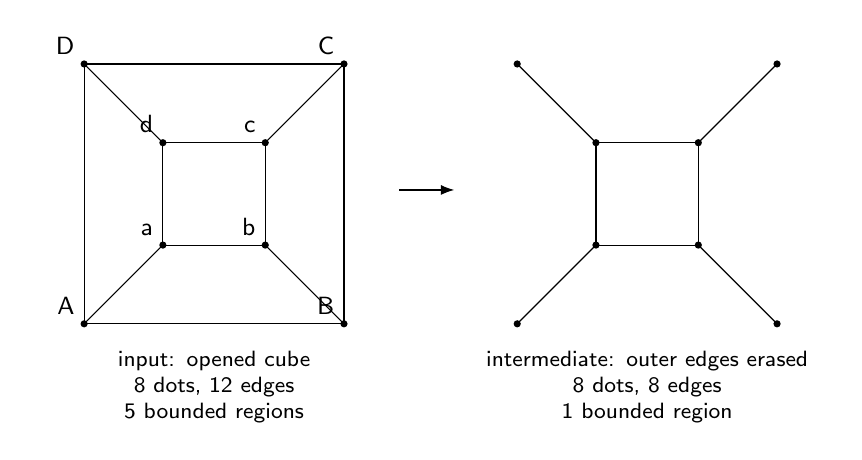
\begin{tikzpicture}[x=1cm,y=1cm,font=\small]
\begin{scope}
\draw (0,0)--(3.3,0)--(3.3,3.3)--(0,3.3)--cycle;
\draw (1,1)--(2.3,1)--(2.3,2.3)--(1,2.3)--cycle;
\draw (0,0)--(1,1) (3.3,0)--(2.3,1) (3.3,3.3)--(2.3,2.3) (0,3.3)--(1,2.3);
\foreach \x/\y/\n in {0/0/A,3.3/0/B,3.3/3.3/C,0/3.3/D,1/1/a,2.3/1/b,2.3/2.3/c,1/2.3/d}{\fill (\x,\y) circle (1.3pt);\node[above left] at (\x,\y) {\n};}
\node[align=center,text width=4.5cm,font=\footnotesize] at (1.65,-.8) {input: opened cube\\8 dots, 12 edges\\5 bounded regions};
\end{scope}
\draw[-{Latex}] (4,1.7)--(4.7,1.7);
\begin{scope}[shift={(5.5,0)}]
\draw (1,1)--(2.3,1)--(2.3,2.3)--(1,2.3)--cycle;
\draw (0,0)--(1,1) (3.3,0)--(2.3,1) (3.3,3.3)--(2.3,2.3) (0,3.3)--(1,2.3);
\foreach \x/\y in {0/0,3.3/0,3.3/3.3,0/3.3,1/1,2.3/1,2.3/2.3,1/2.3}{\fill (\x,\y) circle (1.3pt);}
\node[align=center,text width=4.5cm,font=\footnotesize] at (1.65,-.8) {intermediate: outer edges erased\\8 dots, 8 edges\\1 bounded region};
\end{scope}
\end{tikzpicture}
\end{center}
Erasing $ab$ leaves 8 dots, 7 edges and no bounded regions: a tree. The tetrahedron's printed example erases its three boundary edges, leaving 4 dots, 3 edges and no bounded regions. These deletions also merge with outside; requiring two \emph{bounded} regions would block the displayed route.

\textbf{Why the count is always 2.} Keep deleting cycle edges until none remain. A finite connected graph with no cycles is a tree. A tree has $E=V-1$: remove a leaf and its one edge repeatedly until one dot remains. Therefore its opened count is $V-E+F_{\rm bounded}=V-(V-1)+0=1$. Each earlier deletion removed one edge and one bounded face, preserving that count. Restore the removed face: the closed count is 2. Convexity supplies a plane view through one face with no crossed edges; more generally the same reduction works for a sphere cellulation.

\hints{``Which edge lies on a loop? If you erase it, can its endpoints still reach each other?''}{Try one boundary edge and look at the bounded region joining outside. Keep every dot connected.}{At the final tree, remove leaf dots one by one with their single edges. What relationship survives?}
If graph deletion requires adult control at every step, retain the actual cube experiment as a conjecture and return later to the proof. Children may choose their own legal edges and keep a checkable drawing; they need not reproduce this particular tree.

\newpage
\titleline{Problems 8--9: explain and work backward}
\sub{Problem 8 / student p.8 / deeper continuation}
Children explain the total gap even when vertex types differ. Use the printed pentagon $\rightarrow$ three triangles $\rightarrow$ $540\degc$ example before the general face-angle accounting. The face need not be regular: a plane $n$-gon has angle sum $180(n-2)\degc$. Convex faces triangulate from a corner without outside diagonals; a simple nonconvex polygon also triangulates, but its diagonals need more care.

\textbf{Complete explanation.} Start with one $360\degc$ turn at each of the $V$ vertices. Subtract every incident face angle exactly once. Count those angles face by face instead of vertex by vertex. Across all faces, the side count is $2E$, because every edge belongs to two faces. Subtracting two from each face's side count gives
\[
\begin{aligned}
\hbox{all face angles}&=180\degc\sum_{f}(n_f-2)
 =180\degc(2E-2F)=360\degc(E-F),\\
\hbox{all gaps}&=360\degc V-360\degc(E-F)
 =360\degc(V-E+F)=720\degc.
\end{aligned}
\]
A child can use cards showing each face's angle budget and gather every corner's contribution once; symbolic summation is not required. The essential idea is that rearranging contributions by faces or by vertices does not change their total.

\hints{``On the pyramid, can you account for every face corner once, without grouping equal vertices?''}{``Start with a turn at each vertex. How much do all the faces use? What does a five-sided face use?''}{Pair the two copies of each face side to replace the sum of face-side counts by $2E$; then use the count explained in Problem 7.}
If the angle-sum representation is new, work with actual triangle/square faces first and return to arbitrary $n$. A pattern verified on models remains a conjecture until this reasoning is understood.

\sub{Problem 9 / student p.9 / reverse inventory}
Children use the specified local fan and the whole-solid assumptions to find $(V,E,F)$ without seeing the full solid. Regularity supplies equal face angles; the same number of faces meets at every vertex. They can organize the count with corner tokens rather than simultaneous equations.

\begin{tabularx}{\linewidth}{|p{3.4cm}|Y|}\hline
Five equilateral triangles per vertex & One gap is $360\degc-5(60\degc)=60\degc$. Hence $V=720/60=12$. There are $5V=60$ face-corner incidences: $F=60/3=20$. There are $3F=60$ face sides: $E=60/2=30$. \textbf{$(12,30,20)$}, the regular icosahedron.\\\hline
Three regular pentagons per vertex & A pentagon's angle is $540\degc/5=108\degc$. One gap is $360\degc-3(108\degc)=36\degc$. Hence $V=720/36=20$. There are $3V=60$ corners: $F=60/5=12$; $E=5F/2=30$. \textbf{$(20,30,12)$}, the regular dodecahedron.\\\hline
\end{tabularx}
Both give Euler count 2. The actual existence of these two regular solids is independently checked mathematically; no physical construction of them has been rehearsed or required. These deductions do not show that every locally acceptable fan completes globally, nor classify every possible convex solid.

\hints{``What is the gap in the pictured fan?''}{``If every vertex has that gap, how many copies make two full turns?''}{Count face corners in two ways: faces times corners per face, or vertices times faces per vertex. Pair face sides for edges.}
If division or the 108-degree angle is a barrier, have the adult do the arithmetic the child has chosen. Otherwise set this page aside; retain the reverse question for a later visit rather than replace it with routine angle practice.

\newpage
\titleline{Adult mathematics and return routes}
\sub{A compact map of the proofs}
\textbf{Incidence.} Counting sides over all faces gives $\sum n_f=2E$. Counting face-corner incidences gives the same total, but the multiplicity at a vertex can vary. With exactly $q$ faces at every vertex and exactly $n$ sides per face, $nF=qV=2E$. This is why corner totals alone are insufficient without vertex multiplicities.

\textbf{Euler.} The boundary of a convex polyhedron is a sphere. A view through a removed face gives a connected plane graph with $F-1$ bounded disk regions. Removing a cycle edge preserves connectivity and reduces both edges and bounded regions by one, including when the merged region is outside. Reduction to a tree gives opened count 1, hence closed count 2. A tree's leaf-removal argument proves $E=V-1$. This explains the count; mere agreement among four inventories does not.

\textbf{Angles.} Triangulating an $n$-sided face gives $n-2$ triangles and angle sum $180(n-2)\degc$. Sum the face angles using $\sum n_f=2E$; subtract from $V$ turns. Total defect is $360\degc(V-E+F)=720\degc$. Diagonals preserve old angle sums; new face-center and edge points divide a full turn and have zero defect. Geometric convex corners are positive; subdivisions need not be.

\textbf{The regular-face restriction.} If every face is a regular $n$-gon and $q$ faces meet at every genuine convex vertex, then $n,q\geq3$ and
\[
q\frac{180(n-2)}{n}<360,\qquad (n-2)(q-2)<4.
\]
The integer candidates are $(n,q)=(3,3),(3,4),(3,5),(4,3),(5,3)$. Explicit tetrahedron, octahedron, icosahedron, cube and dodecahedron models establish existence for these cases. The strict inequality excludes flat subdivision vertices. It is a necessary local restriction, not a standalone general assembly theorem. No classification proof is needed to solve Problem 9.

\sub{Several visits from this theme}
\begin{tabularx}{\linewidth}{|p{3.4cm}|Y|}\hline
First concrete visit & Handle closed solids, inventory two or more contrasting models, and try several fans (Problems 1--3). Some groups may reach the gap totals.\\\hline
Unequal and unchanged curvature & Resume Problems 4--6: the pyramid has two vertex types; independently redraw the cube. Invent a new subdivision and predict counts and defects before checking it.\\\hline
Why the totals agree & Pursue the opened graph/tree route (7), then rearrange angle contributions (8). Each deserves its own concrete work. Children can share different spanning trees and check connectivity.\\\hline
Reverse and regular & Use 9, then ask which regular polygon fans can have positive gap. Children sort candidate fans; adults can support the arithmetic. Distinguish restrictions, existence, and a classification argument.\\\hline
Later topology comparison & Revisit the difference between a closed sphere surface and a surface with a boundary, or connect to the existing band investigations. An appropriate holed cellulation needs a separately checked construction before Euler count or signed defects are used.\\\hline
\end{tabularx}
These are different investigations, not a claim that one hour contains the whole theme. Record actual use by problem and readiness, not simply ``Week 56 completed.'' The existing Week 37 tetrahedron work concerns symmetry; Week 26 planar corners and Week 38 bands concern other invariants. Reusing an object need not repeat the mathematical question. Before a return visit, check the use log and the children's saved records rather than infer exposure from library week numbers.

\newpage
\titleline{Source evidence and what to keep}
\sub{Mathematical precedents}
\textbf{Keenan Crane, \emph{Discrete Differential Geometry: An Applied Introduction}.} Exercise 2.1, printed p.22 / PDF p.23, contrasts disk, sphere and genus counts. Exercises 5.9--5.10, printed pp.95--96 / PDF pp.96--97, define angular defect and the discrete Gauss--Bonnet identity. The no-boundary and polygon-incidence assumptions are stated explicitly here. Our elementary face-angle cancellation presentation is an authored derivation.\par
\url{https://www.cs.cmu.edu/~kmcrane/Projects/DDG/paper.pdf}

\textbf{Vicky Neale, NRICH, \emph{Euler's Formula} (February 1, 2011).} The connected planar-graph theorem, edge-removal proof and final polyhedron discussion are precedents for Problem 7. Its rubber-stretching picture is intuition; our proof uses the stated sphere/convex domain.\par
\url{https://nrich.maths.org/articles/eulers-formula}

\textbf{Thomas F. Banchoff, \emph{Beyond the Third Dimension}.} Chapter 5 section 2 compares regular polygon corners around polyhedron vertices; Chapter 6 section 3 discusses Schlegel diagrams. These precede the fan and opened-view ideas.\par
\url{https://www.math.brown.edu/tbanchof/Beyond3d/chapter5/section02.html}

\sub{Teaching evidence, and our adaptation}
\textbf{Givental, Nemirovskaya and Zakharevich, \emph{Math Circle by the Bay}, printed pp.viii--x / PDF pp.9--11:} the authors describe themes with deeper continuations, manipulatives, repeated opportunities to improve explanations, and differing pace/depth. They decline universal topic-duration estimates. This supports flexible routes; it does not validate our session timing.

\textbf{Natasha Rozhkovskaya, \emph{Math Circles for Elementary School Students: Berkeley 2009 and Manhattan 2011}, Lesson 7, ``At the lesson,'' items 1--2:} item 2 reports enthusiastic free polygon construction with K'nex; item 1 reports a group not ready for a triangulation argument and distinguishes a conjecture from an explanation. This is evidence about those sessions, not tested polyhedron-defect pedagogy.

\textbf{Organizer's \emph{Handouts 4.docx}, Problems 4.2--4.5:} physical tiling proceeds to obstruction and symmetry questions; the print-fit note motivates a real dimension check. It supplies no evidence of previous Euler/defect knowledge. The local README/context report children's successful block handling and difficulty retaining paper-only lamp rules. These are organizer-reported observations.

\textbf{Our unpiloted adaptation:} the model choices, fan comparisons, phrasing, figures, launch, exact allocations, hints and routes in this guide are newly authored. Letting children handle objects before counting, keeping state visibly marked, and offering a younger oral fan investigation are reasoned design choices. Arithmetic support must leave the child choosing and testing; it does not establish age fit. Mathematical source attribution is not classroom validation or permission to redistribute downloaded books.

\sub{After the session: an observation, not a verdict}
For each pair/trio, record problems actually attempted, models/fans chosen, who handled/checked/recorded, time spent, and where they want to resume. Save one marked drawing or fan and a child's actual words. Label a claim \textbf{tried}, \textbf{guessed}, \textbf{checked in named cases}, or \textbf{explained}; distinguish ``all four models agreed'' from a general proof.

Record what required help: reading a sentence, arithmetic, aligning corners, remembering closure/no-dents, seeing hidden faces, or selecting the next mathematical action. Note real material fit, tape/marker behavior, assembly/preparation minutes and whether one adult supported both younger pairs. Separate what was observed from a hypothesis about its cause. Use that evidence to adjust the next visit; these pages remain unpiloted until actually used.
\end{document}
